\documentclass[12pt,a4paper]{article}
\usepackage[margin=1in]{geometry}
\usepackage{amsmath,amssymb,bm}
\usepackage{graphicx}
\usepackage{booktabs}
\usepackage{float}
\usepackage{algorithm}
\usepackage{algpseudocode}
\usepackage{hyperref}
\usepackage{siunitx}
\usepackage{tikz}
\usetikzlibrary{arrows.meta,positioning,shapes.geometric}

\title{Methodology: Enhanced Genetic Algorithm with Adaptive Controllers (GAWorker)}
\date{}

\begin{document}
\maketitle

\section{Optimization Problem}
Let $\bm{x} = (x_1,\ldots,x_d)^\top$ denote the decision vector of DVA parameters. For each gene $i$ we have lower/upper bounds $\ell_i, u_i$ and an optional fixed value $c_i$. The feasible set is
\[ x_i = c_i \;\; (i \in \mathcal{F}) , \quad x_i \in [\ell_i,u_i] \;\; (i \notin \mathcal{F}) , \]
where $\mathcal{F}$ is the index set of fixed parameters.

The FRF model maps parameters to a scalar performance indicator (``singular response'') $s(\bm{x};\Theta)$ over a frequency grid $\Omega=[\omega_{\min},\omega_{\max}]$ with $N_\omega$ points, using main system parameters $\Theta$. In addition, target criteria across masses yield percentage differences $\Delta_{m,k}(\bm{x})$ (absolute percent errors) for mass index $m\in\{1,\ldots,5\}$ and criterion $k$.

The scalar fitness minimized by GAWorker is
\begin{equation}
\label{eq:fitness}
f(\bm{x}) = \underbrace{\left| s(\bm{x};\Theta) - 1\right|}_{\text{primary objective}} + \underbrace{\alpha \sum_{i=1}^{d} |x_i|}_{\text{sparsity penalty}} + \underbrace{\frac{1}{S} \sum_{m} \sum_{k} |\Delta_{m,k}(\bm{x})|}_{\text{percentage error term}},
\end{equation}
where $\alpha\ge 0$ is the sparsity weight (named \texttt{alpha} in code) and $S>0$ is a scaling factor (\texttt{percentage\_error\_scale}). The algorithm terminates early when $\min f \le \varepsilon$ (tolerance \texttt{ga\_tol}) or when the generation budget is reached.

\paragraph{Diversity and statistics.} Per generation, GAWorker computes
\[ \mu = \frac{1}{|\mathcal{P}|} \sum_{i\in \mathcal{P}} f_i, \qquad \sigma = \sqrt{\frac{1}{|\mathcal{P}|} \sum_{i\in \mathcal{P}} f_i^2 - \mu^2}, \qquad cv = \frac{\sigma}{|\mu|+\varepsilon}, \]
and a gene-level diversity
\[ D = \frac{1}{d} \sum_{j=1}^{d} \min\!\Big(1,\max\!\big(0, \tfrac{\sigma_j}{u_j-\ell_j}\big)\Big), \]
where $\sigma_j$ is the per-gene standard deviation across the population.

\section{Initialization (Seeding)}
GAWorker supports multiple seeding strategies with fixed-parameter handling:
\begin{itemize}
\item Random: $x_i \sim \mathcal{U}(\ell_i,u_i)$ for unfixed genes, $x_i=c_i$ if fixed.
\item Sobol QMC: sample $\bm{z} \in [0,1]^d$ from a Sobol sequence and scale $\bm{x}=\bm{\ell}+\bm{z}\odot(\bm{u}-\bm{\ell})$; then overwrite fixed genes.
\item Latin Hypercube (LHS): stratified sampling in $[0,1]^d$, then scale to $[\ell_i,u_i]$ and apply fixed genes.
\item Memory seeding: propose from a replay buffer augmented with jitter and exploration.
\item Best-of-pool: generate a large QMC pool, evaluate by \eqref{eq:fitness}, keep best with diversity stride.
\item Neural seeding: propose $\bm{x}$ using a learned surrogate ensemble with acquisition UCB/EI and optional gradient refinement.
\end{itemize}

\paragraph{Why seeding matters (plain language).}
Before evolution begins, we must choose the first ``generation'' of designs to test. Think of seeding as laying different fishing nets across the ocean: better nets (seeding) catch better and more diverse fish (candidate solutions) sooner. Some nets spread widely and evenly (Sobol/LHS), some reuse good past spots (Memory), some try many and keep the best spread-out ones (Best-of-pool), and some use a learned map to suggest promising areas (Neural).

\paragraph{Fixed parameters.}
Sometimes a parameter must stay constant (e.g., a component you cannot change). We enforce that by setting both its lower and upper bound to the same value and keeping it fixed during creation, crossover, and mutation.

\subsection*{Seeding methods explained for newcomers}
\paragraph{Random (uniform inside bounds).}
Like throwing darts blindfolded but making sure you always hit the board: every unfixed parameter is drawn uniformly within its allowed range. Pros: simple and unbiased. Cons: in higher dimensions it may leave big gaps (poor coverage).

\paragraph{Sobol (low-discrepancy) sampling.}
Sobol is a clever way to sprinkle points more evenly than random across a high-dimensional box. Imagine carefully placing dots so that every region gets fair attention. This improves coverage and often speeds up early progress compared to pure random draws.

\paragraph{Latin Hypercube Sampling (LHS).}
LHS divides each parameter range into equal segments and ensures you pick one value from each segment, combining them so that all parameters are well covered. Think of tasting a menu where you try one item from each category, rather than many from just one.

\paragraph{Memory seeding (replay + jitter + explore).}
We keep a lightweight "memory" of past good designs. Memory seeding mixes three ingredients: (i) replay top designs, (ii) add small random tweaks around them (local search), and (iii) add some fresh random points to keep exploring. This provides a strong starting population if you have historical runs.

\paragraph{Best-of-pool (QMC pool + diversity stride).}
We generate a large, well-spread pool (e.g., with Sobol), score them quickly, sort from best to worst, and then pick with a "stride" so selected points are not bunched together. This combines exploitation (use the currently best) with diversity (keep them different) to avoid premature crowding.

\paragraph{Neural seeding (surrogate-guided).}
We train a fast approximation model (a small neural network ensemble) that learns from evaluated designs and predicts which new designs are promising. It balances two goals: (i) try designs that look best (exploitation) and (ii) try designs that reduce uncertainty or add diversity (exploration). This can jump-start the GA with smarter candidates.

\begin{algorithm}[H]
\caption{GenerateSeedIndividuals($n$)}
\begin{algorithmic}[1]
\Require bounds $([\ell_i,u_i])_{i=1..d}$, fixed set $\mathcal{F}$ with values $c_i$, method $M$
\If{$|\mathcal{F}|=d$} \State \Return $n$ copies of $(c_1,\ldots,c_d)$ \EndIf
\If{$M=\textsc{Random}$} \State sample $n$ iid uniformly in bounds, apply fixed genes \State \Return population \EndIf
\If{$M\in\{\textsc{Sobol},\textsc{LHS}\}$}
\State initialize QMC engine for dimension $d$
\State draw $n$ points $\bm{z}\in[0,1]^d$, scale to $[\ell_i,u_i]$, apply fixed
\State \Return population
\ElsIf{$M=\textsc{Memory}$}
\State query memory buffer for $n$ candidates, apply fixed, \Return
\ElsIf{$M=\textsc{Best}$}
\State draw a pool $\mathcal{U}$, evaluate $f(\cdot)$, sort ascending
\State pick $n$ by diversity stride, \Return
\ElsIf{$M=\textsc{Neural}$}
\State propose $n$ via surrogate acquisition (\S\ref{sec:neural})
\State \Return
\Else \State fallback to \textsc{Random}
\EndIf
\end{algorithmic}
\end{algorithm}

\paragraph{Seeding decision tree.}
\begin{center}
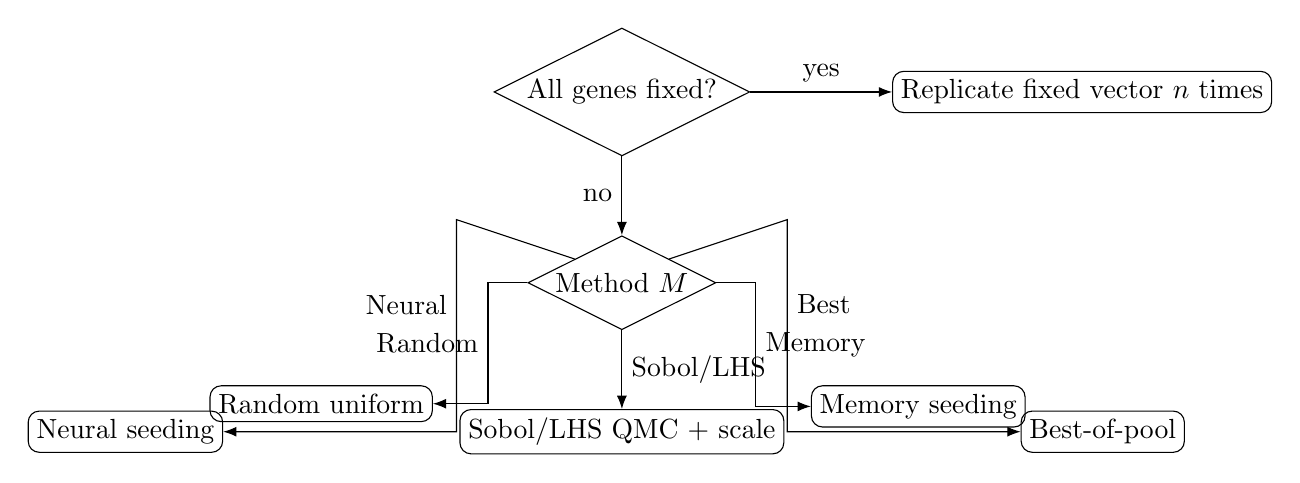
\begin{tikzpicture}[node distance=10mm, line/.style={-Latex}, decision/.style={diamond,draw,aspect=2,inner sep=1pt,align=center}, block/.style={rectangle,draw,rounded corners,inner sep=3pt,align=center}]
\node[decision] (allfix) {All genes fixed?};
\node[block,right=18mm of allfix] (fixed) {Replicate fixed vector $n$ times};
\draw[line] (allfix) -- node[above]{yes} (fixed);
\node[decision,below=10mm of allfix] (method) {Method $M$};
\draw[line] (allfix) -- node[left]{no} (method);
\node[block,below left=10mm and 18mm of method] (rand) {Random uniform};
\node[block,below=10mm of method] (qmc) {Sobol/LHS QMC + scale};
\node[block,below right=10mm and 18mm of method] (mem) {Memory seeding};
\node[block,right=30mm of qmc] (best) {Best-of-pool};
\node[block,left=30mm of qmc] (neural) {Neural seeding};
\draw[line] (method.west) --++ (-5mm,0) |- node[pos=.25,left]{Random} (rand);
\draw[line] (method) -- node[right]{Sobol/LHS} (qmc);
\draw[line] (method.east) --++ (5mm,0) |- node[pos=.25,right]{Memory} (mem);
\draw[line] (method.north east) --++ (15mm,5mm) |- node[pos=.2,right]{Best} (best);
\draw[line] (method.north west) --++ (-15mm,5mm) |- node[pos=.2,left]{Neural} (neural);
\end{tikzpicture}
\end{center}

\subsection{Neural seeding in detail (beginner-friendly)}
\label{sec:neural-detail}
\paragraph{Intuition.}
Evaluating a design is relatively expensive (it runs the FRF and computes targets). A small neural network can learn a quick approximation from the designs we already evaluated. We then ask this learned model where to look next, prioritizing designs that are predicted to be good, while keeping some room to explore unfamiliar regions.

\paragraph{Model (ensemble surrogate).}
We use an ensemble of $M$ small feed-forward networks. Each network takes normalized parameters $\tilde{\bm{x}}\in[0,1]^d$ and outputs a predicted fitness $\hat{f}_m(\bm{x})$. The ensemble provides
\[ \mu(\bm{x}) = \frac{1}{M} \sum_{m=1}^{M} \hat{f}_m(\bm{x}), \qquad \sigma(\bm{x}) = \sqrt{\frac{1}{M-1} \sum_{m=1}^{M} (\hat{f}_m(\bm{x}) - \mu(\bm{x}))^2 }, \]
which we interpret as mean and uncertainty. Architecturally, each network has:
\begin{itemize}
\item Input layer of size $d$ (one neuron per parameter),
\item $L$ hidden layers (e.g., ReLU) with width $H$ and dropout for regularization,
\item A single linear output predicting fitness.
\end{itemize}

\paragraph{Training (fast, incremental).}
Every generation we add the latest evaluated designs $\{(\bm{x}^{(j)}, f^{(j)})\}$ to a training buffer. We normalize inputs to $[0,1]$ using bounds. Each network trains a few short epochs (or up to a time cap) with mean squared error loss $\mathcal{L} = \frac{1}{B}\sum (\hat{f}-f)^2$ on small batches. This keeps training overhead low while adapting to new data.

\paragraph{Acquisition functions (choose where to sample).}
For minimization we support:
\begin{align*}
\text{UCB}(\bm{x}) &= \mu(\bm{x}) - \beta\,\sigma(\bm{x}) && (\beta>0:\; \text{trade-off mean vs. uncertainty}),\\
\text{EI}(\bm{x}) &= \mathbb{E}[\max(0, f^* - F(\bm{x}))] \,\approx\, (f^* - \mu)\,\Phi(z) + \sigma\,\phi(z),\; z=\frac{f^*-\mu}{\sigma},
\end{align*}
where $f^*$ is the best fitness so far, and $\Phi,\phi$ are the standard normal CDF and PDF. UCB is simple and robust; EI directly models expected improvement.

\paragraph{Candidate generation and selection.}
We generate a pool of size $\rho n$ (e.g., using Sobol), enforce fixed genes, and score candidates by the acquisition. We select $(1-\varepsilon)n$ best by acquisition and fill the remaining $\varepsilon n$ by a diversity heuristic (choose points far from those already selected). The exploration fraction $\varepsilon$ can adapt with stagnation: if improvement stalls, we increase exploration to escape local traps.

\begin{algorithm}[H]
\caption{NeuralSeeder: propose($n$)}
\begin{algorithmic}[1]
\Require pool multiplier $\rho>1$, exploration fraction $\varepsilon\in[0,1]$, acquisition $\mathcal{A}(\cdot)$
\State build pool $\mathcal{U}$ of size $\lceil \rho n\rceil$ in $[\ell_i,u_i]$, apply fixed genes
\State score each $\bm{x}\in\mathcal{U}$ by $a(\bm{x})\leftarrow \mathcal{A}(\bm{x})$ (lower is better)
\State $k \leftarrow \lfloor (1-\varepsilon)n\rfloor$; pick $k$ lowest $a(\bm{x})$ to form $\mathcal{S}$
\State while $|\mathcal{S}|<n$: add the point in $\mathcal{U}\setminus\mathcal{S}$ that maximizes distance to $\mathcal{S}$ (diversity)
\State optional: gradient refinement of $\mathcal{S}$ within bounds
\State \Return $\mathcal{S}$
\end{algorithmic}
\end{algorithm}

\paragraph{Neural seeding workflow.}
\begin{center}
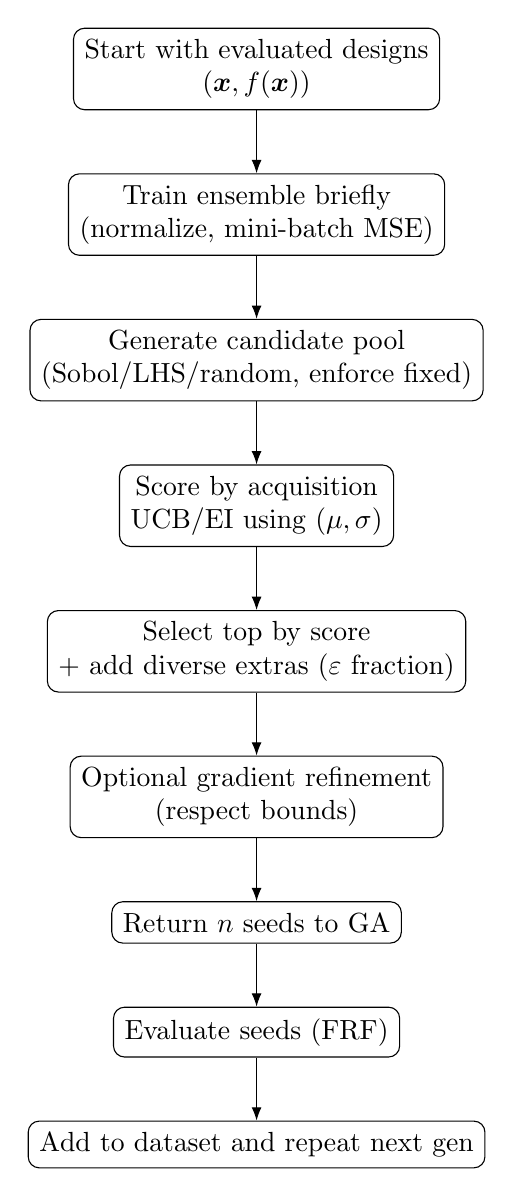
\begin{tikzpicture}[node distance=10mm, line/.style={-Latex}, box/.style={rectangle,draw,rounded corners,inner sep=4pt,align=center}]
\node[box] (data) {Start with evaluated designs\\$(\bm{x},f(\bm{x}))$};
\node[box,below=8mm of data] (train) {Train ensemble briefly\\(normalize, mini-batch MSE)};
\node[box,below=8mm of train] (pool) {Generate candidate pool\\(Sobol/LHS/random, enforce fixed)};
\node[box,below=8mm of pool] (score) {Score by acquisition\\UCB/EI using $(\mu,\sigma)$};
\node[box,below=8mm of score] (select) {Select top by score\\+ add diverse extras ($\varepsilon$ fraction)};
\node[box,below=8mm of select] (refine) {Optional gradient refinement\\(respect bounds)};
\node[box,below=8mm of refine] (seed) {Return $n$ seeds to GA};
\node[box,below=8mm of seed] (eval) {Evaluate seeds (FRF)};
\node[box,below=8mm of eval] (loop) {Add to dataset and repeat next gen};
\draw[line] (data) -- (train);
\draw[line] (train) -- (pool);
\draw[line] (pool) -- (score);
\draw[line] (score) -- (select);
\draw[line] (select) -- (refine);
\draw[line] (refine) -- (seed);
\draw[line] (seed) -- (eval);
\draw[line] (eval) -- (loop);
\end{tikzpicture}
\end{center}

\paragraph{When to use which seeding method?}
\begin{itemize}
\item Use \textbf{Random} for quick tests or low dimensions.
\item Use \textbf{Sobol/LHS} for broad, even coverage when you have no prior data.
\item Use \textbf{Memory} to leverage previous runs or restart from good regions.
\item Use \textbf{Best-of-pool} when you can afford a larger initial screening and want both quality and spread.
\item Use \textbf{Neural} when evaluations are costly and you want the GA to start with informed, high-quality candidates that balance exploration and exploitation.
\end{itemize}

\section{Evolutionary Operators}
\paragraph{Selection.} Tournament selection of size $3$.

\paragraph{Crossover (Blend).} For parents $\bm{x},\bm{y}$ and $\beta\in[0,1]$ (code uses $\beta=0.5$), offspring gene-wise
\[ x'_i = \mathrm{clip}\big(\beta x_i + (1-\beta) y_i,\; [\ell_i,u_i]\big), \quad x'_i \leftarrow c_i\; (i\in\mathcal{F}). \]

\paragraph{Mutation.} With probability $p_{\text{mut}}$ per individual, and per-gene probability $p_{\text{ind}}$ (\texttt{indpb}), apply
\[ x_i \leftarrow \mathrm{clip}\big(x_i + \delta_i,\;[\ell_i,u_i]\big), \qquad \delta_i \sim \mathcal{U}\big(-\eta\Delta_i,\;\eta\Delta_i\big), \]
where $\Delta_i=u_i-\ell_i$ and $\eta$ is the dynamic mutation scale (\texttt{mutation\_scale}). Fixed genes are skipped.

\begin{algorithm}[H]
\caption{One Generation (selection, crossover, mutation, repair)}
\begin{algorithmic}[1]
\State $\mathcal{O} \leftarrow$ clone(\textsc{SelectTournament}$(\mathcal{P},|\mathcal{P}|,t=3)$)
\ForAll{pairs $(o_1,o_2) \in \mathcal{O}$}
\If{\textsc{Rand}() $< p_{\text{cx}}$} \State $(o_1,o_2) \leftarrow$ \textsc{Blend}$(o_1,o_2,\beta)$; repair to bounds, apply fixed \EndIf
\EndFor
\ForAll{$o\in\mathcal{O}$}
\If{\textsc{Rand}() $< p_{\text{mut}}$} \State $o\leftarrow$ \textsc{Mutate}$(o,\eta)$; repair to bounds, apply fixed \EndIf
\EndFor
\State evaluate invalid $o\in\mathcal{O}$ using Algorithm~\ref{alg:evaluate}
\State replace $\mathcal{P}\leftarrow\mathcal{O}$
\end{algorithmic}
\end{algorithm}

\section{Fitness Evaluation}
\begin{algorithm}[H]
\caption{EvaluateIndividual($\bm{x}$)}\label{alg:evaluate}
\begin{algorithmic}[1]
\If{paused/aborted} \State \Return large penalty \EndIf
\State $s \leftarrow$ \textsc{FRF}$(\bm{x};\Theta,\Omega)$; if missing, sum composite measures
\State $f_1\leftarrow |s-1|$; $f_2\leftarrow \alpha\sum_i |x_i|$
\State $E\leftarrow \sum_{m}\sum_{k} |\Delta_{m,k}(\bm{x})|$
\State \Return $f(\bm{x}) = f_1 + f_2 + E/S$
\end{algorithmic}
\end{algorithm}

\section{Adaptive Hyperparameter Control}
Let $(p_{\text{cx}},p_{\text{mut}},N)$ denote crossover prob., mutation prob., and population size.

\subsection{Legacy heuristic (success/diversity driven)}
Maintain an EMA of success rate $\hat{s}$ and gene diversity $\hat{D}$. Every heartbeat or upon stagnation:
\begin{align*}
&\text{if } \hat{s} < 0.9 s^*:\; p_{\text{mut}} \leftarrow \min(\bar{p}_{\text{mut}},\, 1.25\, p_{\text{mut}}),\\
&\text{if } \hat{s} > 1.1 s^*:\; p_{\text{mut}} \leftarrow \max(\underline{p}_{\text{mut}},\, 0.8\, p_{\text{mut}}),\\
&\text{if } D \ll D^*:\; p_{\text{mut}}\uparrow,\; p_{\text{cx}}\downarrow,\; \eta\uparrow;\quad \text{if } D \gg D^*:\; p_{\text{cx}}\uparrow,\; p_{\text{mut}}\downarrow,\; \eta\downarrow.
\end{align*}

\subsection{ML Bandit controller (UCB)}
Define a discrete action set $\mathcal{A}=\{(\delta_{cx},\delta_{mut},\rho)\}$ to scale $(p_{\text{cx}},p_{\text{mut}},N)$. For action $a$, maintain count $n_a$ and average reward $\bar{R}_a$. At time $t$ select
\[ a_t = \arg\max_{a\in\mathcal{A}}\; \underbrace{\big(w_h\,\bar{R}_a + w_c\,R_t\big)}_{\text{blended exploitation}} + c\sqrt{\tfrac{\ln t}{n_a}}. \]
The per-generation reward mirrors the code:
\[ R_t = \frac{\max(0, f^*_{t-1}-f^*_t)}{\Delta t \cdot \max(1,\#\text{evals})} - \lambda\,|cv_t - cv^*|. \]
Apply the selected action as
\[ p_{\text{cx}} \leftarrow \mathrm{clip}\big(p_{\text{cx}}(1+\delta_{cx}),[\underline{p}_{\text{cx}},\bar{p}_{\text{cx}}]\big),\; p_{\text{mut}} \leftarrow \mathrm{clip}\big(p_{\text{mut}}(1+\delta_{mut}),[\underline{p}_{\text{mut}},\bar{p}_{\text{mut}}]\big),\; N\leftarrow \mathrm{round}\,\mathrm{clip}(\rho N,[N_{\min},N_{\max}]). \]

\begin{algorithm}[H]
\caption{ML Bandit step}
\begin{algorithmic}[1]
\State compute $(\mu,\sigma,cv)$ and best $f^*_t$; measure $\Delta t$, evals
\ForAll{$a\in\mathcal{A}$}
\State $U_a \leftarrow (w_h\bar{R}_a + w_c R_t) + c\sqrt{\ln t / n_a}$ (if $n_a=0$ set $U_a=+\infty$)
\EndFor
\State pick $a_t=\arg\max U_a$; update $(p_{\text{cx}},p_{\text{mut}},N)$; resize population if needed
\State after generation: observe $R_t$ and update $\bar{R}_{a_t}$, $n_{a_t}$
\end{algorithmic}
\end{algorithm}

\subsection{RL controller (Q-learning)}
States $s\in\{0,1\}$ encode coarse progress; actions are as above. Epsilon-greedy selection and tabular update
\[ Q(s,a) \leftarrow Q(s,a) + \alpha\,\big[ r + \gamma \max_{a'} Q(s',a') - Q(s,a)\big]. \]
\begin{algorithm}[H]
\caption{RL step}
\begin{algorithmic}[1]
\State with prob. $\varepsilon$ pick random $a$, else $\arg\max_a Q(s,a)$
\State apply $a$, run generation, observe reward $r$ and next state $s'$
\State $Q(s,a)\leftarrow Q(s,a)+\alpha\,[r+\gamma\max_{a'}Q(s',a')-Q(s,a)]$
\State $s\leftarrow s'$, $\varepsilon\leftarrow \varepsilon\cdot\text{decay}$
\end{algorithmic}
\end{algorithm}

\paragraph{Controller decision tree.}
\begin{center}
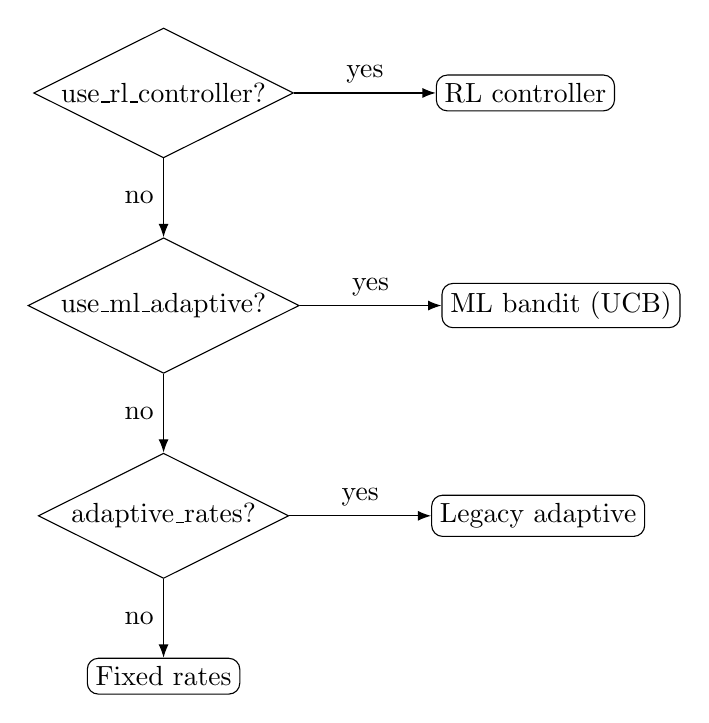
\begin{tikzpicture}[node distance=10mm, line/.style={-Latex}, decision/.style={diamond,draw,aspect=2,inner sep=1pt,align=center}, block/.style={rectangle,draw,rounded corners,inner sep=3pt,align=center}]
\node[decision] (rl) {use\_rl\_controller?};
\node[block,right=18mm of rl] (rlb) {RL controller};
\draw[line] (rl) -- node[above]{yes} (rlb);
\node[decision,below=10mm of rl] (ml) {use\_ml\_adaptive?};
\draw[line] (rl) -- node[left]{no} (ml);
\node[block,right=18mm of ml] (mlb) {ML bandit (UCB)};
\draw[line] (ml) -- node[above]{yes} (mlb);
\node[decision,below=10mm of ml] (adp) {adaptive\_rates?};
\draw[line] (ml) -- node[left]{no} (adp);
\node[block,right=18mm of adp] (adpb) {Legacy adaptive};
\node[block,below=10mm of adp] (fix) {Fixed rates};
\draw[line] (adp) -- node[above]{yes} (adpb);
\draw[line] (adp) -- node[left]{no} (fix);
\end{tikzpicture}
\end{center}

\section{Surrogate-Assisted Screening}
In generations with invalid offspring and sufficient history, GAWorker screens a candidate pool by a $k$NN surrogate in the normalized cube. Let $\tilde{\bm{x}}$ be the normalized vector with $\tilde{x}_i=(x_i-\ell_i)/(u_i-\ell_i)$. For a candidate $\bm{z}$, predict
\[ \hat{f}(\bm{z}) = \frac{1}{k} \sum_{j \in \mathcal{N}_k(\tilde{\bm{z}})} y_j, \qquad y_j = f(\bm{x}^{(j)}), \]
where $\mathcal{N}_k$ indexes the $k$ nearest neighbors among past evaluations. Select $q$ candidates with the lowest $\hat{f}$ (exploitation) and a remainder by maximum novelty (largest minimum distance to the training set).

\begin{algorithm}[H]
\caption{Surrogate screening of invalid offspring}
\begin{algorithmic}[1]
\Require target evaluate count $q$, pool factor $\rho>1$, history $\{(\bm{x}^{(j)},y_j)\}$
\State build pool $\mathcal{U}$ by cloning/mutating/crossover until $|\mathcal{U}|=\lceil \rho q\rceil$
\State compute $\hat{f}(\cdot)$ by $k$NN in $[0,1]^d$; sort $\mathcal{U}$ ascending
\State $q_e\leftarrow \lfloor (1-\xi) q\rfloor$ exploit, $q_x\leftarrow q-q_e$ explore
\State choose first $q_e$ by lowest $\hat{f}$; choose $q_x$ by novelty (max min-distance)
\State evaluate chosen; replace invalid offspring accordingly
\end{algorithmic}
\end{algorithm}

\paragraph{Surrogate decision.}
\begin{center}
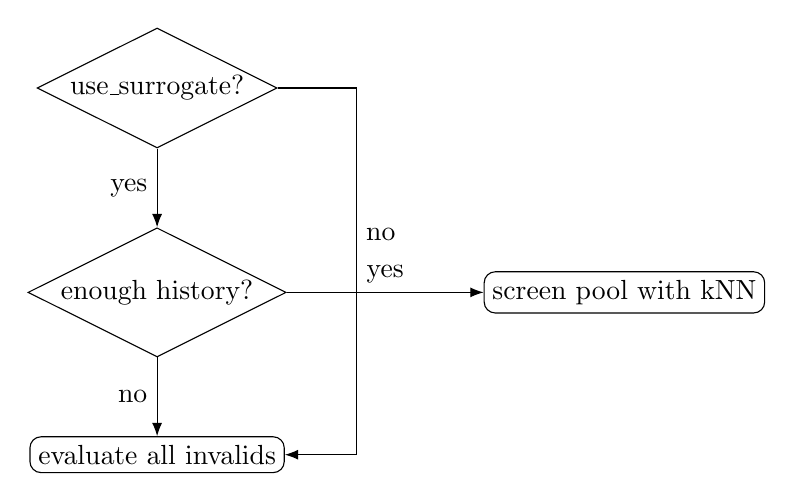
\begin{tikzpicture}[node distance=10mm, line/.style={-Latex}, decision/.style={diamond,draw,aspect=2,inner sep=1pt,align=center}, block/.style={rectangle,draw,rounded corners,inner sep=3pt,align=center}]
\node[decision] (use) {use\_surrogate?};
\node[decision,below=10mm of use] (enough) {enough history?};
\node[block,right=25mm of enough] (screen) {screen pool with kNN};
\node[block,below=10mm of enough] (eval) {evaluate all invalids};
\draw[line] (use) -- node[left]{yes} (enough);
\draw[line] (use.east) --++ (10mm,0) |- node[pos=.2,right]{no} (eval);
\draw[line] (enough) -- node[above]{yes} (screen);
\draw[line] (enough) -- node[left]{no} (eval);
\end{tikzpicture}
\end{center}

\section{Complete Algorithm}
\begin{algorithm}[H]
\caption{GAWorker main loop}
\begin{algorithmic}[1]
\State initialize seeding method and population $\mathcal{P}_0$ (Algorithm 1); evaluate all
\For{$t=1$ to $T$}
\State if paused/aborted: break
\State select controller by decision tree; update $(p_{\text{cx}},p_{\text{mut}},N)$; resize if needed
\State run one generation (selection, crossover, mutation, repair)
\State evaluate invalid offspring; if surrogate enabled and ready, screen first
\State update best-so-far, statistics $(\mu,\sigma,cv,D)$, success rate, EMAs
\State apply adaptive heuristics or controller updates; log metrics
\State if $\min f \le \varepsilon$: break
\EndFor
\State return best individual and full metrics; compute final FRF and report
\end{algorithmic}
\end{algorithm}

\section{Neural Seeding (optional)}\label{sec:neural}
An ensemble surrogate is trained incrementally from $(\bm{x},f(\bm{x}))$ pairs. Acquisition functions include UCB and EI. Given $\beta\in[\beta_{\min},\beta_{\max}]$ and exploration fraction $\varepsilon$ (optionally adapted with stagnation), propose a pool and select by acquisition and diversity; newly evaluated samples augment the training set.

\end{document}
